%
%  Introduction
% ==============
%

\chapter{Introduction}
\label{Ch:Intro}

The Advanced Wakefield Experiment (AWAKE) \cite{awake_collaboration:2014}, located at the old CNGS\footnote{The CERN Neutrinos to Gran Sasso (CNGS) experiment was operational between 2006 and 2012.} facility at CERN, became operational in December 2016. It is a proof-of-concept Proton Driven Plasma Wakefield Accelerator (PDPWFA) using the proton beam from the Super Proton Synchrotron (SPS) as its drive beam.

AWAKE is currently in Run 1 where the interaction between the proton drive beam and the plasma will be studied, and where a long electron witness beam will be injected to sample the wakefields. Run 2 is planned to start after the next Long Shutdown of the LHC (LS2) scheduled for 2019 and 2020, when significant upgrades will be made to the experiment. Run 2 will attempt to accelerate a short, intense electron beam to high energy while avoiding growth in emittance and large energy spread. In preparation for Run 2, a number of design choices needs to be made based on the results of Run 1 as well as simulations of Run 2. The work presented in this thesis primarily focuses on the beam loading of a short electron witness beam through simulations, in preparation for AWAKE Run 2.

The key results are presented in Publication \ref{Pub:BL17}, with the studies leading up to this presented in two conference papers: Publication \ref{Pub:IPAC15} and \ref{Pub:NAPAC16}. A third conference paper, Publication \ref{Pub:IPAC17}, covers the integration of the AWAKE experiment with the CERN control system, which is the main contribution to Run 1 in this PhD project.

In this chapter we will first cover some of the key concepts involved in plasma wakefield acceleration techniques relevant to the work presented in this thesis. The design of the AWAKE experiment itself is laid out in more detail in the next chapter, and the framework for the simulations is described in the third chapter. The fourth chapter outlines the work done in integrating AWAKE Run 1 with the control system at CERN.

% ================================================================================================ %
\section{Plasma Wakefield Acceleration}
\label{Int:PWFA}

Accelerating particle beams in a plasma is an attractive concept as plasmas are capable of sustaining significantly higher accelerating fields than RF structures used in conventional accelerators can. Such RF structures suffer electrical breakdowns at very high electric fields, and these breakdowns can over time damage the structures \cite{braun:2003}. This puts an upper limit on the accelerating gradient of about $350$ to $400\unit{MV/m}$. As these breakdowns causes damage to the surfaces of the RF cavities, in practice the upper limit is determined by the statistical probability of a breakdown and the acceptable number of breakdowns in a given period of time \cite{pritzkau:2002}, and the practical limit is therefore lower.

While RF cavities use standing electromagnetic waves to accelerate particles, plasma accelerators use an energetic beam to drive strong electromagnetic wakefields in the plasma. The two main techniques for producing these strong accelerating fields are by the use of an intense laser beam, or by the use of a particle drive beam. Laser accelerator techniques were investigated in the early 1970s \cite{chan:1971, palmer:1972}, and wakefield acceleration techniques through the use of computer simulations at the end of the decade \cite{tajima:1979}. Using particle beams to drive accelerating wakefields were proposed some time later, in 1985 \cite{chen:1985}.

Both these beam and laser driver techniques utilise a neutral plasma where the collective motion of the free electrons define the main parameters of the accelerating structure. The characteristic time of the electron motion is related to the plasma frequency, $\omega_{pe}$, and the characteristic length is related to the plasma wavelength, $\lambda_{pe}$.
\begin{equation}
    \lambda_{pe} = \frac{2\pi c}{\omega_{pe}}, \quad
    \omega_{pe}  = \sqrt{\frac{n_{0}e^{2}}{m_{e}\epsilon_{0}}}, \label{EQ:PWFA:L0W0}
\end{equation}
where $n_{0}$ is the initial plasma electron density, $e$ is the elementary charge, $m_{e}$ is the electron mass, and $\epsilon_{0}$ is the vacuum permittivity \cite{tonks:1929, esarey:1996, pecseli:2012}. Here we ignore the ion mass and we assume the plasma is cold, i.e. we ignore the thermal motion of the electrons. The characteristic time and length of ion motion scales as the square root of the mass difference compared to the plasma electrons and tend, depending on the ion mass, to be a few orders of magnitude longer than those of the electrons. In the case of very long accelerating structures, the motion of the ions may become an issue.

Plasmas can in general sustain accelerating electric fields on the order of the non-relativistic wave-breaking field \cite{dawson:1959, esarey:1996}
\begin{equation}
    E_{\mathrm{WB}} = \frac{m_{e} c \omega_{pe}}{e}. \label{EQ:EWB}
\end{equation}
For instance, for a plasma density of $10^{18}\unit{cm}^{-3}$, the maximum field is on the order of $100\unit{GV/m}$. This has been inferred by experiment in the mid 1990s when a few electrons was accelerated to over $40\unit{MeV}$ in about $300\unit{\mu m}$ of Helium plasma, driven by a $25\unit{TW}$ pico second laser \cite{modena:1995}.

Both techniques require a drive beam that deposits energy into the plasma in the form of wakefields. The drive beam is trailed by another beam which draws energy from the fields in order to accelerate. We thus see a transfer of energy from the drive beam to the witness beam through plasma as the intermediate medium \cite{muggli:2009}. Let us briefly introduce the core principle of the two methods of plasma wakefield acceleration. 

% ================================================================================================ %
\subsection{Laser Driven Acceleration}
\label{Int:LWFA}

In a laser wakefield driven plasma accelerator (LWFA), the plasma acts like a transformer, changing high frequency transverse field of the laser pulse into a low frequency longitudinal wave \cite{malka:2009}. The effect driving the accelerating fields was described by Tajima and Dawson in 1979, and can be summarised as follows: The ponderomotive force at the front of the laser pulse drives plasma electrons forward, while at the back of the pulse it pushes them backwards. This generates a longitudinal wave that is at its most efficient when the length of the laser pulse $L_{ph} = \lambda_{pe}/2$ \cite{tajima:1979}. The longitudinal field is then loaded by a trailing particle beam to be accelerated, or in some instances plasma electrons are being captured and accelerated instead.

% ================================================================================================ %
\subsection{Beam Driven Acceleration}
\label{Int:BDPWFA}

In a beam driven plasma wakefield acceleration (PWFA) a drive beam of charged particles are sent through a section of neutral plasma. The space charge of the drive beam displaces the plasma electrons, which oscillate at the plasma frequency, creating periodic regions of low and high electron density generating strong wakefields. The longitudinal and transverse fields generated by this wake is then loaded by a trailing beam of particles. The principles behind this technique were formulated in the 1980s by Pisin Chen \emph{et al.} \cite{chen:1985}.

Any type of charged particle beam can be used in such an accelerator. Most experiments to date have used electrons. It has been shown that energy can be transferred from one or more electron drive beams to a single electron witness beam in multiple past experiments \cite{rosenzweig:1988, blumenfeld:2007, kallos:2008, litos:2014}. In one experiment at the Stanford Linear Accelerator Center (SLAC), a $42\unit{GeV}$ electron beam passing through an $85\unit{cm}$ section of ionised Lithium vapour, saw the trailing part of the electron beam reach $85\unit{GeV}$. This corresponds to a gradient of $52\unit{GV/m}$ \cite{blumenfeld:2007}.

A limitation using an electron beam with a similar initial charge and energy for both drive and witness beams is that the witness beam will rapidly gain energy, while the drive beam loses energy. This both causes the drive beam to quickly decelerate, while the witness beam undergoing acceleration will at the same time catch up with the drive beam. Typically propagation length of an electron drive beam is a few tens of centimetres of plasma.

% ================================================================================================ %
\section{Beam-Plasma Interaction}
\label{Int:BPI}

As a beam propagates through plasma, it affects the local density of the plasma electrons. A positively charged beam will pull plasma electrons towards the propagation axis, while a negatively charged beam will push them away \cite{lee:2001,adli:2016b}. Plasma electrons expelled from the axis by a negative beam will be pulled back by the relatively stationary ions. When these electrons are pulled towards the axis by a positive charge from ions or a beam they overshoot, resulting in a oscillating system. Tne magnitude of these oscillations are determined by the beam current, and the oscillation period by the plasma wavelength. If the current is sufficiently large, electrons are completely expelled from the axis, forming a \textit{bubble} \cite{hogan:2016,muggli:2017}. An illustration of an electron beam travelling though a plasma is shown in Figure \ref{Fig:PWFA:Illust}.

\begin{figure}[hbt]
    \centering
    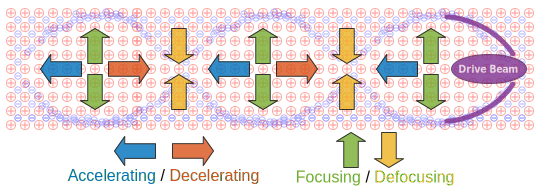
\includegraphics[width=0.85\linewidth,trim={0mm 0mm 0mm 0mm},clip]{figures/PlasmaWakefield}
    \caption{\label{Fig:PWFA:Illust} Illustration of a plasma wakefield accelerating structure with a single electron drive beam. A series of focusing/defocusing and accelerating/deceleratring regions (as seen for an electron witness beam) are produced behind the drive beam.}
\end{figure}

% ================================================================================================ %
\subsection{The Linear Regime}
\label{Int:BPI:Lin}

When the charge density of the beam is smaller than that of the plasma, the system is in the \textit{linear regime}. 

[Add stuff from Patric's \cite{muggli:2017}]

A point like charge travelling at a speed close to the speed of light, will generate fields in its wake \cite{van_der_meer:1985, chen:1985}:
\begin{align}
    E_{z} &= -\frac{Q_{b}k_{pe}^{2}}{2\pi\epsilon_{0}} K_{0}(k_{pe}r)\cos(k_{pe}z - \omega_{pe}t) \label{EQ:PWFA:EZ} \\
    E_{r} &= \hphantom{-} \frac{Q_{b}k_{pe}^{2}}{2\pi\epsilon_{0}} K_{1}(k_{pe}r)\sin(k_{pe}z - \omega_{pe}t), \label{EQ:PWFA:ER}
\end{align}
where $Q_{b}$ is the charge of the beam, $k_{pe}$ is the plasma wave number, and $K_{0}$ and $K_{1}$ are modified Bessel functions. 

Cite \cite{ruth:1985}

% ================================================================================================ %
\subsection{The Non-Linear Regime}
\label{Int:BPI:NLin}

In the non-linear regime, also referred to as the \textit{blowout} regime in the literature, the plasma electrons are expelled from the region around the axis to form a region populated by only plasma ions. As the ions are practically stationary on the time scale of the plasma electrons, they form a uniform column of positive charge. The electrons displaced by the space charge of the drive beam are pulled back on axis by the ions, within the characteristic time $\omega_{pe}^{-1}$, to form a thin sheath of electrons with the shape of a bubble \cite{lu:2006a,lu:2006}. Hence, this is also sometimes referred to as the \textit{bubble} regime.

A conceptual illustration of an electron beam driven plasma accelerator is shown in Fig. \ref{Fig:PWFA:Illust}. Several regions of decreasing magnitude of accelerating/decelerating and focusing/defocusing are generated behind the drive beam. By positioning a trailing beam in an optimal phase, such a beam can both accelerated and focused. The drive beam needs to be shorter than the plasma period for this structure to develop, but multiple short drive beams with a separation of the plasma wave length can amplify the wakefields.

% ================================================================================================ %
\section{Protons vs. Electrons as Drive Beam}
\label{Int:PDPWFA}

Further details on proton driven plasma wakefield goes here.

Benefit of larger energy per bunch, challenge of producing short bunches.

Cite \cite{adli:2016a}.

% ================================================================================================ %
\section{The Self-modulation Instability}
\label{Int:SMI}

A long beam with respect to the plasma wavelength will generate a density wave driven by its own head. This is true for both laser beams \cite{esarey:1994} and particle beams \cite{kumar:2010}, and they are caused by the same underlying physics. For a laser beam, this produces alternating regions of focusing and diffraction. For a particle beam, the wakefields generated within the beam acts back on itself, breaking it up into short micro bunches with a surrounding, defocused halo.

In the 1980s, this self-modulating effect was taken advantage of in LWFA experiments as only long laser pulses were available. Advances in ultra short laser technology later removed the dependence of this effect \cite{pukhov:2002}, however for proton drive beams this is still an issue. For instance, the SPS proton beam used by AWAKE is orders of magnitude longer than the plasma wavelength needed for the experiment.

The self-modulation instability (SMI), is one of several instabilities affecting long beams in plasma.

% To add: Phase velocity of SMI WF. Two-stream and hosing.

In electron beam \cite{muggli:2014}.

% ================================================================================================ %
\section{Numerical Simulations of PWFA}
\label{Int:Sim}

PIC codes. Osiris vs, QuickPIC.

Numerical Cherenkov, Lehe. Relevance to emittance.

Reference to PIC appendix.

Maybe something about resolution and convergence.

% ================================================================================================ %
